\documentclass[aspectratio=169]{beamer}

\usepackage[utf8]{inputenc}

\usepackage{amssymb}
\usepackage{color}
\usepackage{listings}
\usepackage{tikz}
\usepackage{hyperref}
\usepackage[normalem]{ulem}

\usetheme{Rochester}
\usecolortheme{beaver}

\addtobeamertemplate{navigation symbols}{}{%
    \usebeamerfont{footline}%
    \usebeamercolor[fg]{footline}%
    \hspace{1em}%
    \insertframenumber/\inserttotalframenumber
}

\lstloadlanguages{C++}
    \lstset{%
        language={C++},
        basicstyle=\ttfamily,
        keywordstyle=\color{blue},
        showstringspaces=false,
        escapechar={§},
        escapeinside=||
    }

\newif\iftransitions
 \transitionstrue


\newif\iffast
% \fasttrue

\title{Random Numbers Are Hard(er Than You Think)}
%\subtitle{Lua for C++ Programmers}
\author{Andreas Weis}
\institute{BMW AG}
\date{Meeting C++ 2019}
%\titlegraphic{
\includegraphics[height=.25\textheight]{resources/cppcon.png}}


\begin{document}

\frame{\titlepage}

\iffalse
\begin{frame}[fragile]
  \frametitle{About me}

  \begin{itemize}
    \setlength\itemsep{1.5em}

    \item \href{https://stackoverflow.com/users/577603/comicsansms}{
\includegraphics[height=.05\textheight]{resources/so-icon.png}} \href{https://github.com/ComicSansMS}{
\includegraphics[height=.05\textheight]{resources/github-icon.png}} 
\includegraphics[height=.05\textheight]{resources/slack-icon.png} ComicSansMS

    \item \href{https://twitter.com/DerGhulbus/}{
\includegraphics[height=.05\textheight]{resources/twitter-icon.png} @DerGhulbus}

    \item 
\includegraphics[height=.05\textheight]{resources/meetup-icon.png} Co-organizer of the \href{https://www.meetup.com/MUCplusplus/}{Munich C++ User Group}

    \item Currently working as a Software Architect for BMW 
\includegraphics[height=.1\textheight]{resources/bmw_group.jpg}

  \end{itemize}
\end{frame}
\fi

\iffalse
\begin{frame}[fragile]

  \frametitle{Let's build a casino...}

  \begin{lstlisting}


srand(time(NULL));

auto roll_die = []() { return (rand() % 6) + 1; };
  \end{lstlisting}

\end{frame}


\begin{frame}
\frametitle{Does this give good results?}

Nobody knows\ldots

\end{frame}
\fi

\begin{frame}[fragile]

  \frametitle{Let's build a casino!}

  \begin{lstlisting}

std::random_device rdev;
std::mt19937 eng{rdev()};

auto roll_die = [&eng]() {
  std::uniform_int_distribution<int> dist(1, 6);
  return dist(eng);
};
  \end{lstlisting}

\end{frame}

\iffalse

\begin{frame}
\frametitle{What makes a good random number generator?}

\begin{itemize}
  \item Uniform distribution
  \item Unpredictable
\end{itemize}

\end{frame}

\fi

\begin{frame}[fragile]

\frametitle{People must not be allowed to cheat the casino}

\begin{lstlisting}
static long next;
int rand(void) {
    next = next * 1103515245 + 12345;
    return (int)(next/65536) % 32768;
}
\end{lstlisting}

\pause

\begin{lstlisting}
std::cout << std::mt19937::state_size
          << sizeof(std::mt19937::result_type);
\end{lstlisting}

\pause

\begin{semiverbatim}
\$ ./a.out
624 4
\end{semiverbatim}

$\Rightarrow 19968$ bits of state in the engine.
\end{frame}


\begin{frame}[fragile]

  \frametitle{So, we're all good?}

  \begin{lstlisting}
std::random_device rdev;
std::mt19937 eng{rdev()};
  \end{lstlisting}

\pause

  \begin{lstlisting}
std::cout << sizeof(decltype(rdev()));
  \end{lstlisting}

\pause
\begin{semiverbatim}
\$ ./a.out
{\color{red}4}
\end{semiverbatim}

Uh-oh...


\end{frame}

\begin{frame}

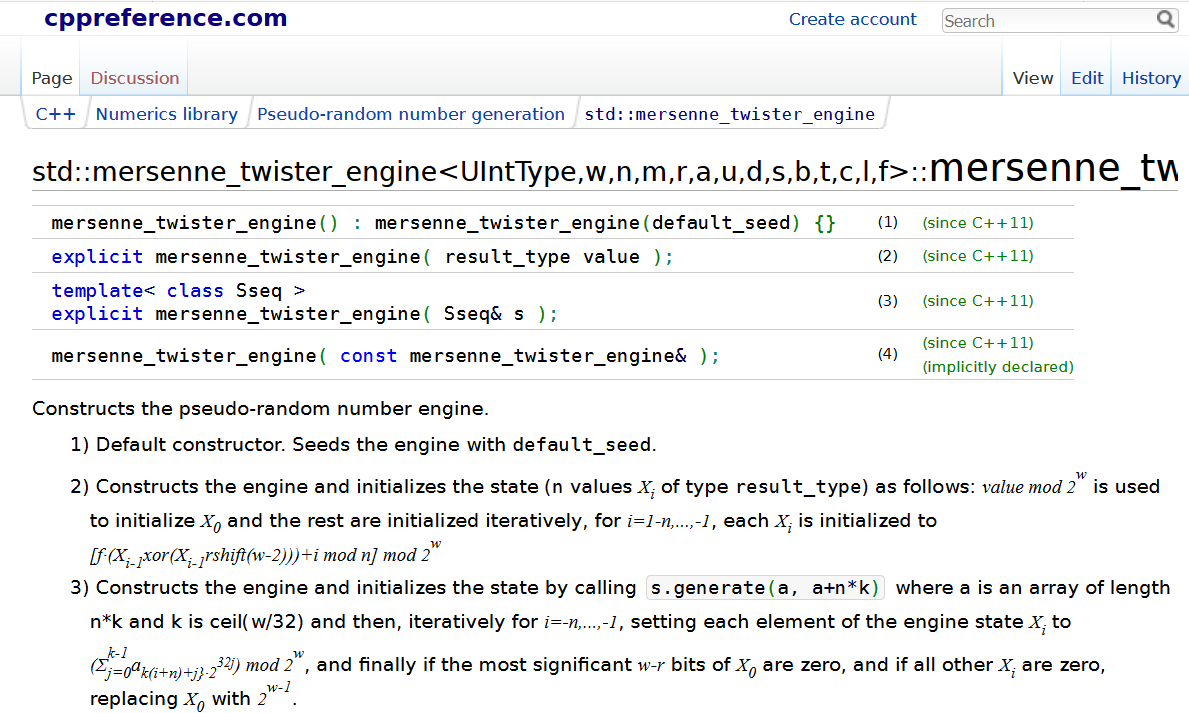
\includegraphics[height=1.0\textheight]{resources/mersenne_cppref.png}

\end{frame}

\begin{frame}

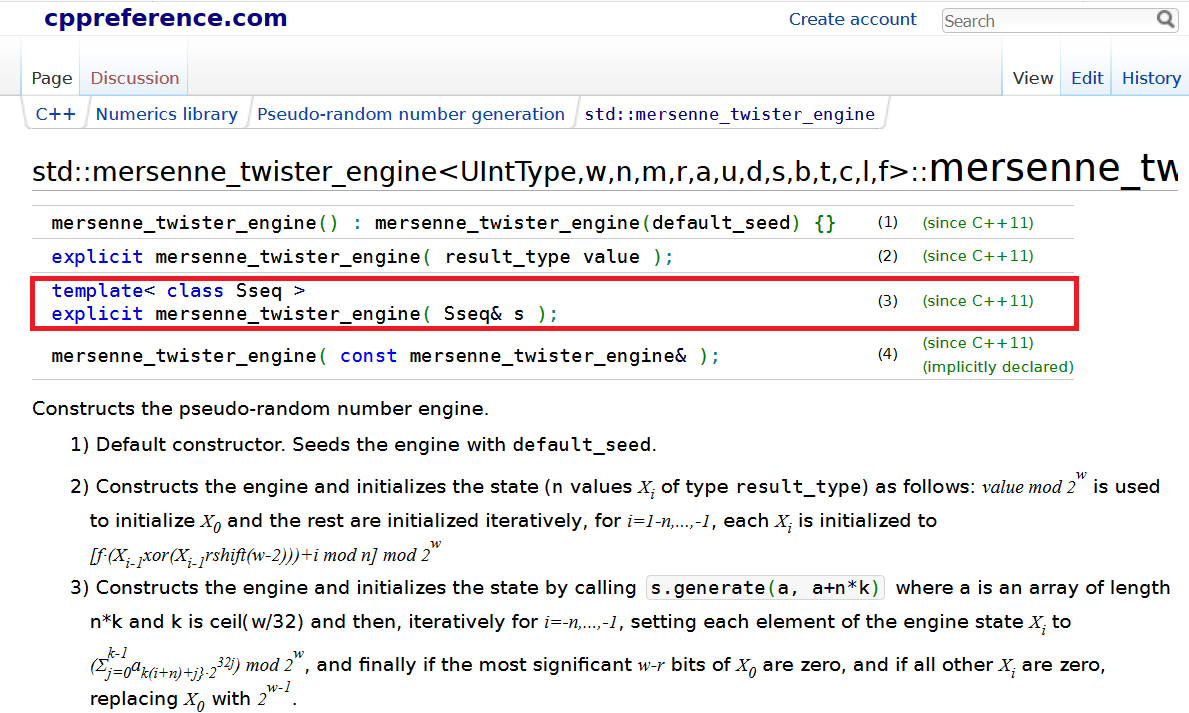
\includegraphics[height=1.0\textheight]{resources/mersenne_cppref_highlighted.png}

\end{frame}

\begin{frame}

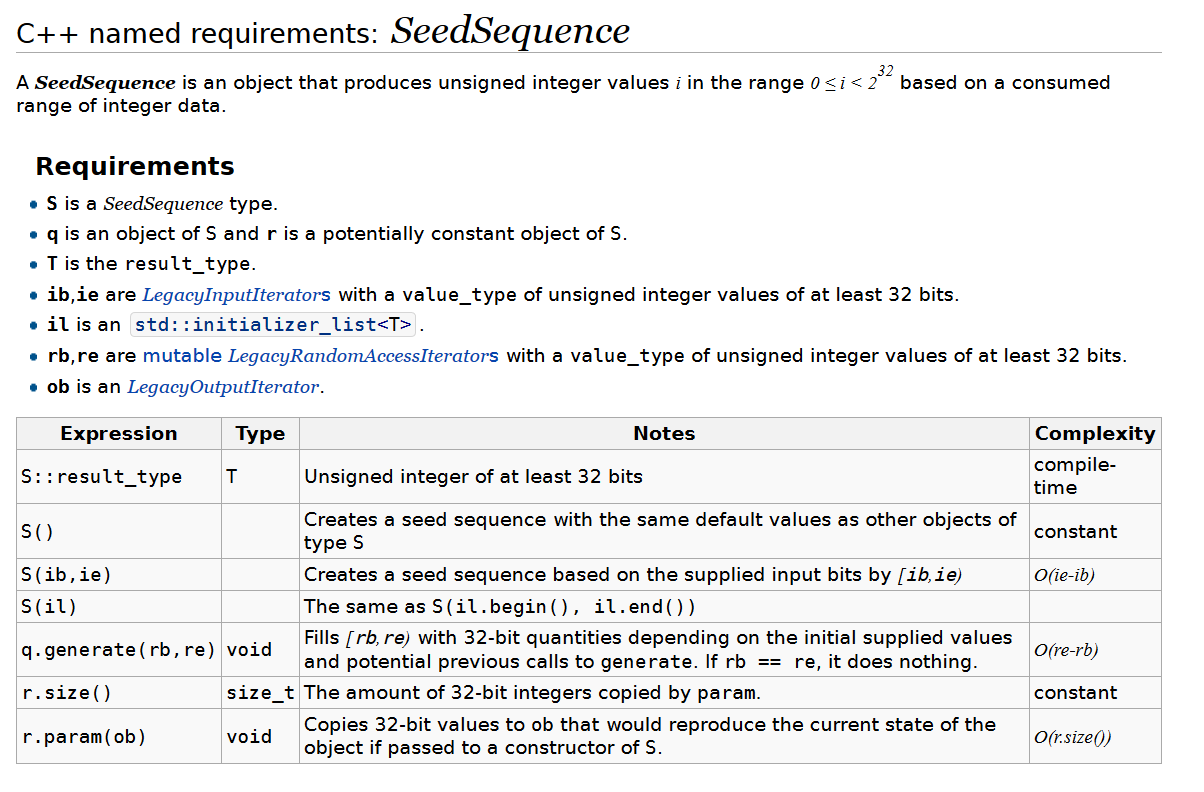
\includegraphics[height=1.0\textheight]{resources/seedsequence_cppref.png}

\end{frame}


\begin{frame}[fragile]
\frametitle{Seeding from a SeedSequence}

\begin{semiverbatim}
{\color{blue}struct} MySeedSequence \{
  {\color{blue}using} result_type = {\color{blue}unsigned int};
  {\color{blue}template}<{\color{blue}typename} It>
  {\color{blue}void} generate(It rb, It re)
  \{


  \}
\};
MySeedSequence seq;
std::mt19937 rng(seq);



\end{semiverbatim}
\end{frame}


\begin{frame}[fragile]
\frametitle{Seeding from a SeedSequence}

\begin{semiverbatim}
{\color{blue}struct} MySeedSequence \{
  {\color{blue}using} result_type = {\color{blue}unsigned int};
  {\color{blue}template}<{\color{blue}typename} It>
  {\color{blue}void} generate(It rb, It re)
  \{
    std::cout << std::distance(rb, re) << " "
      << {\color{blue}sizeof}({\color{blue}typename} std::iterator_traits<It>::value_type);
  \}
\};
MySeedSequence seq;
std::mt19937 rng(seq);



\end{semiverbatim}
\end{frame}


\begin{frame}[fragile]
\frametitle{Seeding from a SeedSequence}

\begin{semiverbatim}
{\color{blue}struct} MySeedSequence \{
  {\color{blue}using} result_type = {\color{blue}unsigned int};
  {\color{blue}template}<{\color{blue}typename} It>
  {\color{blue}void} generate(It rb, It re)
  \{
    std::cout << std::distance(rb, re) << " "
      << {\color{blue}sizeof}({\color{blue}typename} std::iterator_traits<It>::value_type);
  \}
\};
MySeedSequence seq;
std::mt19937 rng(seq);

\$ ./a.out
{\color{red}624 4}
\end{semiverbatim}
\end{frame}


\begin{frame}[fragile]

  \frametitle{Seed Sequence from a \texttt{random\_device}}

  \begin{semiverbatim}
{\color{blue}struct} LotsoRandomSeedSequence \{
  {\color{blue}using} result_type = {\color{blue}unsigned int};
  {\color{blue}template}<{\color{blue}typename} It>
  {\color{blue}void} generate(It rb, It re)
  \{
    std::random_device rdev;
    std::generate(rb, re, [&]() \{ return rdev(); \});
  \}
\};

LotsoRandomSeedSequence seq;
std::mt19937 rng(seq);
  \end{semiverbatim}

\end{frame}


\begin{frame}
\frametitle{This is almost legal...}
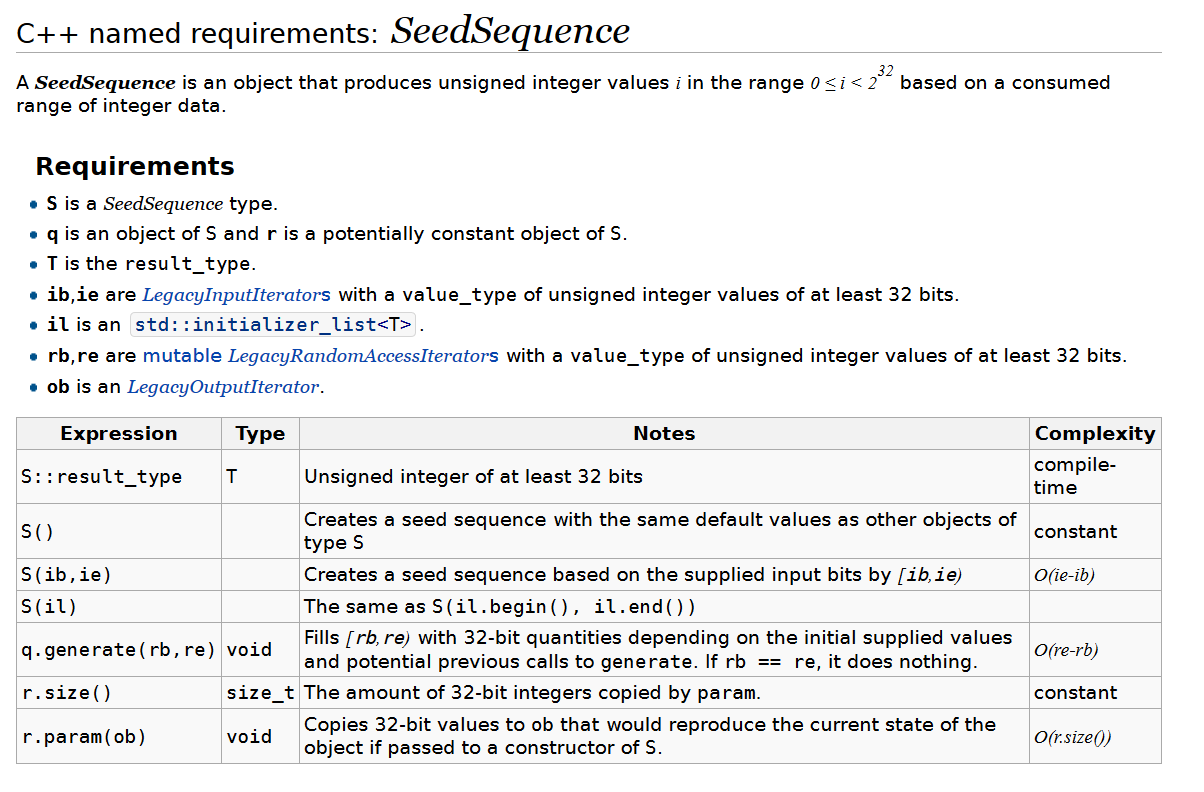
\includegraphics[height=1.0\textheight]{resources/seedsequence_cppref.png}

\end{frame}


\begin{frame}
\frametitle{References}

\begin{itemize}
    \item \href{https://wg21.link/p0205r0}{P0205 - Allow Seeding Random Number Engines with \texttt{std::random\_device}}
    \item \href{http://www.pcg-random.org/categories/c\%2B\%2B.html}{Melissa E. O'Neill's blog (pcg-random.org)}
\end{itemize}

\end{frame}


\begin{frame}[fragile]
  \frametitle{Thanks for your attention}

  \begin{itemize}
    \setlength\itemsep{1.5em}

    \item \href{https://stackoverflow.com/users/577603/comicsansms}{
\includegraphics[height=.05\textheight]{resources/so-icon.png}} \href{https://github.com/ComicSansMS}{
\includegraphics[height=.05\textheight]{resources/github-icon.png}} 
\includegraphics[height=.05\textheight]{resources/slack-icon.png} ComicSansMS

    \item \href{https://twitter.com/DerGhulbus/}{
\includegraphics[height=.05\textheight]{resources/twitter-icon.png} @DerGhulbus}
  \end{itemize}
\end{frame}


\end{document}
